% Chapter 1

\chapter{Architecture Overview} % Main chapter title

\label{Chapter1} % For referencing the chapter elsewhere, use \ref{Chapter1} 

\lhead{Chapter 1. \emph{Architecture Overview}} % This is for the header on each page - perhaps a shortened title

%----------------------------------------------------------------------------------------

\section{Introduction}

In safety critical systems it is sometimes necessary to use redundancy to ensure that the output from a processor is valid. The most common method of building a system with redundancy today is called lockstep execution or dual modular redundancy (DMR). In DMR, the entire processor core is replicated and outputs from store instructions are kept in a buffer until it can be verified that the data and addresses of both cores match. There are several disadvantages related to the scalability of lockstep execution given in \cite{lafrieda2007utilizing}:
\begin{itemize}
\item The temperature and energy requirements for lockstep cores are very high because "DMR pairs running code with similar power/thermal characteristics are necessarily placed next to each other on the die."
\item It is not possible for the cores to execute independently. This also means that if there is a permanent fault in one core, then neither core can be used.
\item The performance of the cores must be very precise and kept synchronized at the level of individual instructions (although there is often a small delay between thread executions on the order of tens of instructions).
\item Core pairs with different frequency or leakage characteristics are bounded by the performance of the slower core.
\item The cummulative effect of the previous items make it difficult to envision a practical and scalable multicore solution to redundancy that relies mainly on lockstep for all resources.
\end{itemize}
The advantages of lockstep include:
\begin{itemize}
\item The detection of errors requires no software intervention or supervision.
\item Code requires no special modifications to be ported onto a lockstep architecture.
\item There is no significant impact on the predictability or execution time of code on the DMR pair compared to a single core.
\item Error correction by voting can be accomplished by increasing the amount of redundancy.
\end{itemize}

Some sections of this thesis (mainly Chapter 1 and Chapter 5) are also being submitted as part of a conference paper.

\subsection{Scalable alternatives to lockstep execution}

\textit{Fingerprinting} is one of many possible alternatives or evolutions to lockstep and DMR. The main insight behind fingerprinting is that it is possible to compare hashes or fingerprints (FPs) calculated based on the activity of a processor core (execution stream or ES) rather than directly comparing the ES itself. The ES in its simplest form consists of store addresses and data however it can also include load addresses and changes to the register file. 

Fingerprinting has been an important component of several proposed architectural features over the last decade that demonstrated promising preliminary results in simulation. These features attempt to resolve the limitations of lockstep DMR that make it difficult to scale with the number of cores of an MPSoC. 

Another feature of commonly predicted in future distributed embedded systems is a \emph{mixed criticality} workload. Mixed criticality is "the integration of applications of different criticality (safety, security, real-time and non-real time) in a single embedded
system" \cite{perez2013safety}. Besides possible high level advantages that can emerge from improved allocation of resources, integrating distributed systems onto a single chip can improve the amount of wiring in a system dramatically. It is claimed in \cite{swingler2000degradation} that 30-60\% of automotive system failures are attributable to interconnect failures. 

System features related to the improvement of resource allocation and application scheduling are:
\begin{itemize}
\item \textit{On-Demand Redundancy:} One natural target for increasing efficiency is to allow cores to be able to execute independent tasks or applications in parallel when redundancy is not required. It is wasteful to run an application that does not require redundancy on a pair of cores in lockstep. Ideally, applications could monitor critical tasks and detect errors with redundancy services provided by the system while allowing less critical tasks to run independently and concurrently on the two cores.
\item \textit{Dynamic Core Coupling (DCC):} Consider attempting to derive a static schedule for several applications on an MPSoC with six or eight cores where redundancy services are available on-demand. One possibility is to provide redundancy services in hardware by allowing three pairs of cores to execute in lockstep. Again, intuitively, an optimal solution is more likely to be found if \textit{any} two cores can be paired in lockstep and if these pairings can be adjusted at runtime. Previous simulation work on DCC has shown much better schedules can be derived when this is the case.
\end{itemize}

In order to provide the flexibility of DCC a system must be able to monitor the ES, establish a sphere of replication (SoR) by which errors are contained and not allowed to contaminate main memory, and provide a mechanism for comparing the ES of different cores independently of interconnect topology. Software and hardware overhead related to the management of monitoring resources must be kept to a minimum. As previous authors have noted, hardware monitoring of the ES is preferable but the amount of information required to compare the ES of different cores must be reduced. Fingerprinting is an important component to designing a system with these characteristics. 

The integration of partitioning and resource allocation through hypervisors and health-monitoring services such as those proposed for the monitor core in the ACROSS platform provide an interesting starting point for the development of a comprehensive fault tolerance strategy aimed at multicore platforms. While we are not yet able to either duplicate or integrate a hypervisor, we can allow them to inform our design choices.

\begin{figure}[h]
\centering
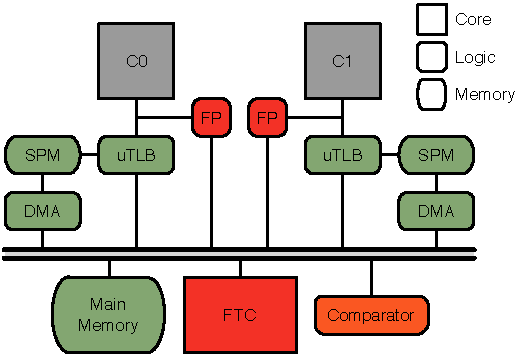
\includegraphics[scale=1.5]{Figures/architecture}
\caption{System view of hardware platform.}
\label{f:arch}
\end{figure}

We propose a novel system implementing heterogeneous reliability, presented in Figure \ref{f:arch}, that provides the necessary hardware functionality to support dynamic core coupling and on-demand redundancy, and broaden the scope of design-space exploration for reliability-constrained cost optimization.
	We have designed the required logic, written simple drivers, and demonstrated the ease with which fingerprinting can be integrated into a traditional RTOS environment.	
	This architecture utilizes:
\begin{itemize}
\item	\emph{Fingerprinting logic} to compress modifications to external state into a single, fixed-width word;
\item	\emph{Scratch-pad memories, $\mu$TLBs, and DMAs} to manage modified state under quarantine until redundancy checking has been performed on corresponding fingerprints;
\item	Scalable \emph{comparison logic} to identify and compare matching fingerprints when their corresponding instructions segments have finished executing; and
\item	A \emph{fault-tolerant core} to execute safety-critical tasks, and coordinate the activity of the above units to safely monitor critical tasks executing on unreliable processors.
\end{itemize}
	The above hardware can be unintrusively integrated with the host processor system, and requires no modification to the processor core or compiler.
	When not needed, redundancy checking may be disabled, freeing resources to perform other tasks independently and therefore improving performance relative to lockstep execution (under which redundancy checking is continually performed)~\cite{Meyer:CASES11}.
	
\section{Related Work}
\subsection{The ACROSS MPSoC}


The ACROSS MPSoC was a joint project of 16 European partners from industry and academia. It is a comprehensive multicore architecture combining time triggered network fabric and up to ten cores to provide reliable and deterministic application execution \cite{el2013across}. A recent expansion of the project has been the automatic design space exploration of a reliable embedded system. Models of the application and platform are used to explore the design space of application to resource mappings that take into account reliability and timing requirements. The system automatically generates application source code and platform configuration files \cite{huang2014framework}. Their analysis of of reliable design space exploration  is independent of a specific method of detecting errors. The performance overhead associated with a fault tolerance mechanism are simply another parameter in the platform model that will inform the search for an optimal allocation of resources. 


%The ACROSS MPSoC is at the center of a large project that aims to demonstrate a highly predictable multicore architecture for safety-critical and general real-time multicore distributed systems. The project has proceeded to using platform modelling to generate distributed application code for the entire system based on performance parameters.The criticality of an application is one such parameter used to determine if a task should be replicated on several cores. However, while the existence of several proposed mechanisms for capturing and comparing the ES are known, there is yet to be a realistic architectural solution that that can be implemented with current technology. This platform is such an architecture and we borrow heavily from the ACROSS project. Many assumptions made about parts of the system that have yet to be implemented are based on results stemming from the ACROSS project.

One key feature of the ACROSS platform is the reservation of certain cores for monitoring the rest of the system \cite{kopetz2007automotive}. One of the special cores is the \textit{diagnostic core} which uses information from local \textit{health monitoring services} belonging to the general purpose cores to detect anomalies. We believe this vision for distributed multicore platforms to be very promising and that fingerprinting can play an important role in monitoring services in such a platform for mixed-criticality applications requiring redundancy. 

Taken from Huang et al. \cite{huang2014framework}:
\begin{quote}
Our approach is based on the following:
\begin{itemize}
\item Platform-independent description of the application including timing and reliability requirements.
\item Fine-grained platform model covering both hardware platform
and system software (HW/SW stack).

\item Multi-criteria design space exploration: mapping and scheduling w.r.t. timing and reliability constraints (consideration of
permanent and transient faults).
\item Automatic insertion of fault-tolerance techniques, including
active redundancy, voting and fault detection to meet userspecified reliability goals.
\item Generation of implementation artifacts such as application C
source code and platform configuration files.
\end{itemize}
\end{quote}

Their work deliberately avoids committing to a specific fault tolerance mechanism: 
\begin{quote}
The configurability enables the user to select candidate FTMs for
the specific application domain and is therefore essential for the
practical applicability of the approach.
\end{quote}

An ideal fault tolerance mechanism for such a system would be easily managed and customized by software, provide a high degree of flexibility and configurability in terms of error detection strength, and rely on dedicated hardware to minimize the performance impact of monitoring the system. It would also be independent of network or bus topology and place minimal restrictions on scheduling strategies (i.e. it would have minimal impact on an optimization solution that assumes zero overhead). Fingerprinting can be easily viewed as a fine-grained \emph{health-monitoring service} used by the monitor to ensure safe operation of critical tasks.

\subsection{The Xtratum Hypervisor}

Another project that represents significant progress on related issues is the Xtratum hypervisor that is designed for hardware paravirtualization (hardware resources are only partially virtualized to minimize performance overhead in real-time systems) of  and safely implementing mixed criticality systems with provable partitioning mechanisms in place. We have currently only implemented enough software architecture to demonstrate how fingerprinting could be built into an RTOS at the lowest level. We rely on projects such as Xtratum as proof of the types of services that could be integrated with these low level functionalities to provide more developed task replication services making for a sort of plug-and-play DCC. 

The main consideration when it comes to mixed criticality systems and industrial certification is given by Perez et al. in \cite{perez2013safety}:
\begin{quote}The integration of applications of different criticality (safety,
security, real-time and non-real time) in a single embedded
system is referred as mixed-criticality system. This integrated
approach can improve scalability, increase reliability reducing
the amount of systems-wires-connectors and reduce the overall
cost-size-weight factor. However, safety certification according
to industrial standards becomes a challenge because sufficient
evidence must be provided to demonstrate that the resulting
system is safe for its purpose. Higher safety integrity functions
must be interference free with respect to lower safety integrity
functions.
\end{quote}

\subsection{Heterogeneous Reliability}
As with many current trends in embedded systems, the problem of heterogeneous reliability has previously been proposed in the high performance domain \cite{hruby2013slower,he2003reliability,ungsunan2009improving}. Bolchini and Miele explicitly introduce the notion of heterogeneous reliability into the problem of model-based design space exploration for embedded systems \cite{bolchini2013reliability}. They map mixed-criticality applications onto platforms with cores of varying degrees of fault tolerance in terms of strength and cost. They observe that systems with heterogeneous reliability mechanisms can generally provide a wider range of options in terms of optimizing resource utilization given a mixed criticality workload.

Reliability aware scheduling is complex even in the static case due to the need for contingency schedules. In the case where cores are only equipped with the capability to detect but not correct errors, it is necessary to have alternative schedules to reallocate resources so that the critical task deadline is not missed. If several concurrent errors are to be supported, then several branches of contingency schedules are required. In \cite{bolchini2013reliability} it is assumed that tasks can be grouped in order to minimize the amount of software voting tasks required. This creates a tradeoff between voting overhead and detection latency. They assume that the voting overhead should be minimized since errors are rare. 

With fingerprinting, the cost of verifying redundant task executions is completely offloaded into hardware and detection latencies are reduced dramatically. This could eliminate the need for task grouping and simplify the job of developing contingency schedules. If a task within a group fails, then this is only known once the final task in the group completes and the entire group must be rescheduled. With fingerprinting, the amount of work that must be re-executed in the case of an error or errors is reduced dramatically since only a single task is corrupted.

\section{Motivating Example: Scheduling}
\label{s:schedulingstudy}

	Recent work has examined automated design space exploration to map applications onto heterogeneous multicore platforms \cite{bolchini2013reliability,huang2014framework}. 
	We do not address in this work the problem of characterizing the optimal ratio between fault tolerant and plain cores or the possible dependency of this ratio on the application. 
	Figure \ref{f:schedule} shows an example task graph for a set of critical tasks as well as a pool of unrelated non-critical tasks.  
	The platform in question consists of one fault tolerant core and 4 plain cores with fingerprinting units. 
	The benefits of ODR should be apparent right from time 0 since four non critical tasks are able to execute concurrently. 
	As for DCC, consider what happens at time 700. There is only one non-critical task (NCT) remaining once critcal task (CT) 3 is complete. 
	Meanwhile, CT4 cannot begin until time 900 when CT2 is also completed. 
	Core 3 remains busy until time 900 on NCT-d. 
	By allowing C2 and C3 to execute CT4, C1 is freed up to begin executing NCT-f immediately. 
	This example has been successfully implemented using Nios II cores on an Altera Arria FPGA development board using synthetic tasks with matching run times and fingerprinting to verify correct execution.


\begin{figure}[tb]
\centering
\subfloat[]{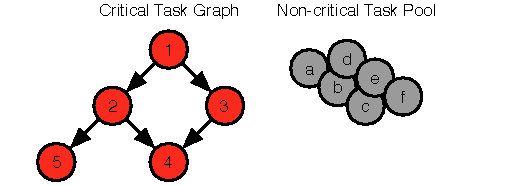
\includegraphics{figures/schedule-tg}} \\
\subfloat[]{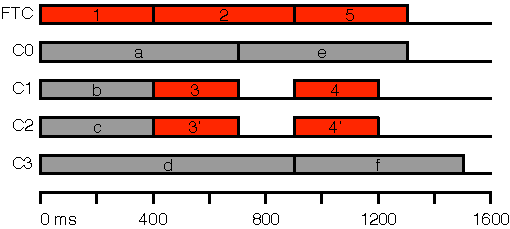
\includegraphics{figures/schedule-nodcc}} \\
\subfloat[]{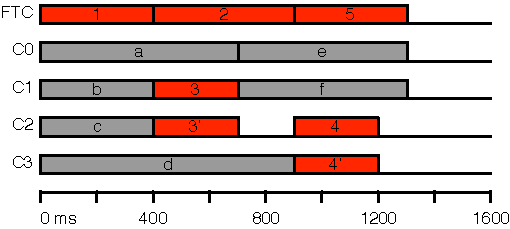
\includegraphics{figures/schedule-dcc}}
\caption[An example task graph for a mixed-criticality system]{(a) The task graph for a sequence of dependent critical tasks and a pool of non-critical tasks to be executed during the same window. (b) The tasks are mapped to a platform without DCC. (c) With DCC, NCT-f can begin 20 ms earlier.}
\label{f:schedule}
\end{figure}

\section{Fingerprinting Architecture}

\subsection{Overview}

The rest of this section will be organized as follows:
\begin{itemize}

\item{List the requirements a fault tolerant mechanism (FTM) should have in the context of an MPSoC with several independent cores.}
\item{Present the main components of the hardware platform.}
\item{Present the organization of a flexible software architecture.}
\item{Examine how each of the requirements is addressed with the high level specification in mind.}
\end{itemize}



\subsection{System Requirements}
This architecture aims to showcase the features of a fault tolerance mechanism that is purposefully suited to the scenario of a multicore RISC processor that uses some combination of specialized hardware and software to ensure predictable and dependable behaviour for mixed criticality applications. Examples of such systems have been discussed in the previous two sections. The future of software designs for such platforms is projected to involve the automatic generation of code as an optimization problem using platform models and various system requirements. This fault tolerant mechanism should therefore have a few basic properties:
\begin{itemize}
\item{Area overhead should be kept to a minimum and must be competitive with DMR or nMR}
\item{Any additional hardware should be scalable with the number of cores in a platform.}
\item{The system should not be dependent on network or bus topology}
\item{Monitoring of the execution stream or other core state information should be implemented in hardware and off the critical data path}
\item{The relative amount of data required to verify correct execution should be small compared to other system bus or network traffic. }
\item{Parameters related to reliability that impact the previously listed properties should be tunable. Tunability will minimize restrictions on the model-based design space exploration when generating optimized application code for a platform.}
\item{At least one agent in the system is permanently reliable and is responsible for monitoring less reliable agents}
\item{There should be a strategy for impeding the propagation of errors to other concurrent tasks on the core or elsewhere in the system}
\item{There should be a path to support the development of low cost checkpointing strategies}
\item{The system should bear some resemblance to DMR as a well established path to certification already exists}
\item{Minimal restrictions should be placed on the software organization in terms of scheduling}
\end{itemize}

\subsection{Hardware Architecture}

The baseline platform in Figure \ref{f:arch} consists of the following elements:
\begin{itemize}
\item{Two cores capable of executing non-critical tasks independently and of loosely synchronizing and executing the same critical tasks in parallel}
\item{Local scratchpads with identical addresses. The scratchpads are currently reserved for critical task stacks and input data however more complex dynamic allocations could be used. }
\item{DMA that can access the scratchpads and main memory. The monitor core is able to set the DMA units}
\item{Fingerprinting units that monitor each core}
\item{A specialized comparator core for collecting and comparing fingerprints from each core}
\item{A monitor core that is assumed to be made reliable through other permanent internal mechanisms that are not visible to the rest of the system (such as DMR). The monitor core is responsible for scheduling tasks and receives updates from the comparator core upon failure or success of a fingerprinted task.}
\end{itemize}


The general control flow for the system is depicted in Figure \ref{f:control_flow}.
	First, the Monitor task on the FTC \encircle{1}~assigns a pair of redundant critical tasks (SW) to two cores.
	This task is executed inside of a wrapper that \encircle{2}~sets up the fingerprinting unit (FP), requesting the software-specified fingerprinting block size for this task.
	Next, \encircle{3}~the task begins, prompting \encircle{4}~the fingerprinting unit to notify the comparator that fingerprint generation has started.
	While the task executes, \encircle{5}~fingerprints are generated and sent to the comparator.
	%As matching fingerprints arrive from the redundant critical task, the comparator compares them.
	As matching fingerprints arrive from the redundant critical task, they are checked by the comparator.
	In the meantime, speculative changes to state are quarantined in a scratch-pad memory (SPM) managed by the Monitor task on the FTC, with the assistance of DMA.
	
	If there is an interrupt and a higher-priority critical needs to execute, fingerprinting \encircle{6}~is paused, and a context switch performed.
	When the higher priority task finishes, control is returned to the original critical task, and fingerprinting is \encircle{7}~resumed.
	%The fingerprinting unit itself need not be aware that this has occurred (Section~\ref{s:hwsw:fingeprinting}).
	The comparator does not require notification that this has occurred.
	The critical task will eventually \encircle{8}~notify the fingerprinting unit that  the task has ended.
	The fingerprinting unit \encircle{9}~communicates this to the comparator, which then \encircle{10}~forwards final voting results to the monitor task. In the case of mismatched fingerprints, the comparator notifies the MC immediately.
%	If there has been an error, the monitor \encircle{11}~communicates this back to software (likely through the operating system) so that corrective action can be taken.
	If there has been an error, the monitor \encircle{11}~ should initiate a contingency schedule so that corrective action can be taken \cite{bolchini2013reliability}.
\begin{figure}[h]
\centering
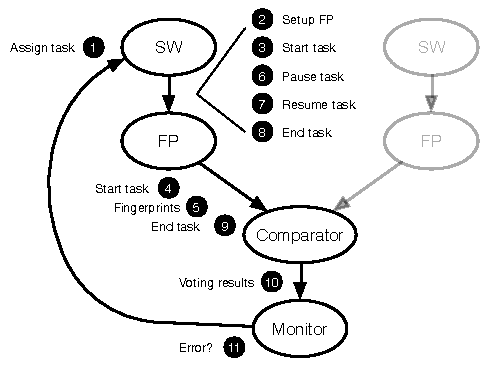
\includegraphics[scale=1.3]{Figures/interfaces}
\caption{System view of hardware platform.}
\label{f:control_flow}
\end{figure}

\subsection{Software Architecture}
 
This section explores the system-wide architectural implications that may arise in the software design due to the limitation of hardware resources and the fundamental requirement of fingerprinting that a task can be deterministically executed on separate cores not just in terms of the result produced but at the fine grain of individual store commands. These issues, pertaining to high level software design, will not be explored in any further detail in this work. However, they present interesting directions to explore in future work.

\subsubsection{Fingerprint task IDs}
Although a more comprehensive justification for the features of the software architecture must wait until the hardware constraints have been explored in more detail, the general organization of critical tasks across the system can still be provided. To begin with, there must be the definition of system wide fingerprint task IDs (FIDs). The maximum number of FIDs will be constrained by the fingerprinting hardware available in the system. This constraint leads naturally to the worry that more critical tasks exist than there are FIDs, making it impossible to statically assign a single FID to each critical function. The assignment of FIDs must be taken into account as another parameter when developing a schedule for the system. This can be easily achieved in a schedule with non-preemptive execution of critical tasks. A different strategy is required in systems where a fingerprinted task may be preempted.

A \emph{fingerprinting window} represents a certain mapping of FIDs to critical tasks. A fingerprinting window can be very short or very long and is meant to organize the assignment of FIDs to guarantee that all critical tasks concurrently executing in a system have an FID available to them. It can represent a static assignment or a static series of assignments. Suppose that the capacity of the system is \emph{n} FIDs. This means that at any given point in time, the comparator hardware is only able to maintain information on \emph{n} tasks at a time. In a system where critical tasks cannot be preempted (not an unreasonable assumption in highly critical real-time systems with very precise deadlines) this is very simple to do, especially if the number of regular cores $p \leq 2n$. For instance, suppose $n = 16$. In a non-preemptive schedule, it is possible to have 16 \emph{pairs} of cores executing a critical task simultaneously.

The fingerprinting window becomes more restrictive in a system that allows preemption of fingerprinted tasks. In this case, more than one critical task may be simultaneously executing on each core. Therefore care must be taken that an FID is available for any task requiring fingerprinting. We can compromise by placing some restrictions on the servicing of these tasks into set frames where no more than 16 functions have access to the fingerprinting resources at a time. Resource sharing in multicore systems with real-time deadlines is an ongoing area of research. Frames or windows are a common theme in establishing predictability of execution making this an approach that could easily be integrated into such a system.

The assignment of functions to FIDs as well as the assignment of FID/function pairs to cores is handled by the reliable monitor core. The monitor core has unique access to the input data for the critical task. Memory protection must be used to guarantee that only the monitor can initiate writes to these addresses (either directly or using DMA). The monitor can then use DMA to prepare the state on the scratchpad on each local core, including input data, function code location, and FID. 

\subsubsection{Deterministic execution}

The \emph{scratchpad resources} of each core are important to ensuring deterministic execution of redundant tasks as well as another limited resource that must be taken into account when scheduling. Both these issues will now be elaborated on. The availability of a stripped down memory virtualization capability may also be required as a practical matter depending on the specific architecture and compiler. 

The \emph{deterministic execution} of a function in a system without virtual memory support and high level process services from the OS is not an unsolvable or even particularly complicated problem but it is also not a forgiving one. Depending on the processor architecture and compiler options available, it can be tricky to generate machine code for one core that can be executed without-modification by another core.

The goal is to allow the compilation of deterministically executing of code without the availability of position independent code options (-fpic) that can be run by any core in the system without modifying the compiler. The issue is that if the code references global variables, then only one copy of the variable exists. There are two less than ideal solutions to this problem. The first is to rewrite the code so that all recurring global state variables used by a function are accessed through pointers passed into the context as function arguments and therefore placed on the stack, and then popped off the stack back into main memory at the end of the execution. The addresses of these variables will never be compiled directly into the machine code of the critical tasks. This can obviously be cumbersome, especially considering that code generated from models may not behave this way. The second is to place copies of global variables in the local scratchpads and use \emph{memory virtualization} to ensure that the references to these variables are rerouted to the local copy.

In order to have strictly deterministic execution of regularly compiled code, all store addresses and data (at a minimum) must match for the entirety of the fingerprinted interval. As a result, it is necessary that the stack pointers match from the beginning of fingerprinting. It is also required that same copy of the code is run from the same address on both cores so that all return addresses pushed onto the stack are matching. It bears repeating that these conditions are restrictive in terms of the way code must be written to guarantee deterministic execution \emph{without} the availability of memory virtualization in a bare-metal (RTOS-based) system. It also bears repeating that virtualization hardware is very central to the design of hypervisors and should be fairly common in embedded real-time MPSoCs. We have include a low cost uTLB for minimal virtualization of scratchpad addressing.

\subsubsection{Fault containment strategies}
	While executing a safety-critical task, the output from unreliable cores are prevented from making changes to external state until such changes have been verified through fingerprint comparison. 
	There are two potential approaches. Firstly, the use of local scratchpad memories or locked caches can be used to store temporary copies of data. 
	Alternatively, several redundant copies could be kept in main memory \cite{dobel2012operating}. 
	In either case, there is a probability that the setting of the MPU is itself corrupted. Either a fault tolerant core should manage memory protection to guarantee that erroneous write addresses cannot corrupt data outside of the current task. In \cite{huang2014framework} it is suggested that a probabilistic argument can be made about the likelihood of that specific task failing to determine whether or not this function must be moved to an FTC. 
	There is no way to guarantee that a failure does not corrupt other tasks concurrently stored on the local memory resource if a non reliable core manages its own local memory protection since the memory protection itself could be erroneously set. 
	In the case of several copies in main memory a single core could reasonably be expected to control a global MPU. 
	We have yet to integrate memory protection strategies into our software development but note that work exists to address certifiable memory partitioning in mixed criticality multicore systems using hypervisors \cite{perez2013safety}.
	
	Advantages of using a scratchpad include not requiring several copies of the data and stack for a critical task in main memory as well as other known benefits including including more deterministic execution \cite{suhendra2005wcet} and energy efficiency \cite{steinke2002assigning}. 
	The difficulty is that there is now another limited resource to be allocated and that will affect scheduling. Furthermore, programs that operate on large data arrays provide problems for scratchpad allocation \cite{francesco2004integrated}. 
	By contrast, keeping several copies in main memory solves many of these problems, however, introduces problems of scalable determinism as the number of cores increases and interference affects memory response times \cite{abel2013impact}. 
	For these reasons, and due to promising work that suggests many of these large data processing algorithms will be shifted to fault tolerant tightly coupled processor arrays \cite{nelis2014challenge,lari2014massively,ferreira2014adaptive}, we will use scratchpads.
	\begin{figure}[h]
\centering
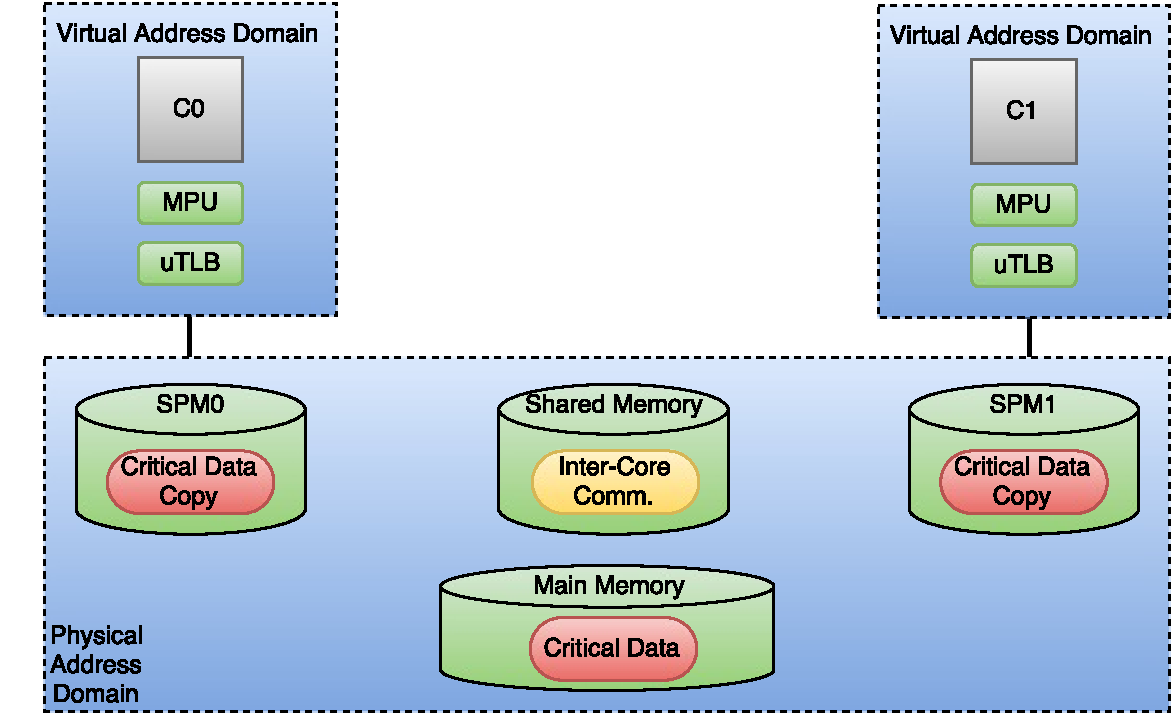
\includegraphics[scale=1]{Figures/sor}
\caption[Memory protection and fault containment]{Memory protection could be used to quarantine changes to critical state in the scratchpad. Less space is required in main memory since the replicas only exist temporarily in the scratchpad. The fingerprint units (FP) base their calculations on the virtual addresses.}
\label{f:sor}
\end{figure}
	Figure \ref{f:sor} shows how memory partitioning can be used to create temporary copies of critical data in scratchpads and protect the original in main memory. It should not be possible for the plain cores to access protected data directly.
	Both the critical task stacks and any input data must be protected.
	
	The software is organized using generic critical task wrappers that can execute an arbitrary function with an arbitrary FID.
	The wrapper tasks will either determine from a static schedule or from a message from an FTC when they should execute, what the identify of the critical function is, and where to find its arguments. 
	There should be enough wrapper functions to support the maximum number of concurrent critical tasks expected to run. 
	If there is sufficient room in the scratchpad to store all of the stacks then they can be statically allocated. 
	Otherwise, the stacks for the tasks can be copied into the scratchpad and the uTLB used for address translation. 
	In order for fingerprinting to operate correctly, the virtual addresses of the stack must be identical on both cores. 
%	We simplify the situation by making the scratchpads only addressable locally, and giving them all identical addresses. 
	%This eliminates the need for address translation with static allocation of the scratchpad . 
	The FTC is able to differentiate between these scratchpads using a local single threaded DMA controller.




\subsubsection{Preempting Critical Tasks}
\label{s:hwsw:preemption}

	At times it may be necessary for one critical task to preempt another.
	In the context of fingerprinting, this presents additional challenges:
		the fingerprinting of the preempted task must not be disrupted, but the fingerprinting logic must be available for the new task.
	The simplest solution to the problem is to have the software notify the hardware when it begins servicing an interrupt. 
	The problem arises that there is no way for communication between software and hardware to occur without the software corrupting its own context (it must load the address of the hardware into a register). 
	We propose a convention whereby the fingerprinting hardware is able to roll back its calculations by one iteration, thus allowing a single store instruction to be executed without corrupting the fingerprint. 
	When an interrupt occurs, the initial context saving assembly routine is modified to store exactly one register onto the stack, and then this register is used to load the address of the fingerprint unit pause strobe. 
	The fingerprint unit rolls back its calculation by one iteration when it receives the pause strobe. 
	When the fingerprint process resumes, the execution streams from both cores will still match.
	
	It is possible to imagine more complex message passing between the OS and the fingerprinting unit once fingerprinting has been successfully paused. 
	For instance, the fingerprinting unit currently only supports rate monotonic scheduling and stores paused task context on a stack. 
	It is reasonable for the OS to pass messages to the fingerprinting to notify it which task is being resumed and for the hardware stack to be replaced by a more flexible data structure. 
	There are potential issues here in that the unreliable core is now passing information to the FP unit that may affect the fingerprinting of several tasks if it is not done properly. 
	We do not explore this issue in any greater detail but note that this behaviour is easily supported by the hardware should it be desired.
In order for the system to provide fail operational capabilities it must be shown that any erroneous executions are not able to contaminate other tasks or applications. It will be necessary to implement a fine grained memory protection strategy. This aspect of the problem has not yet been explored for this project. 
